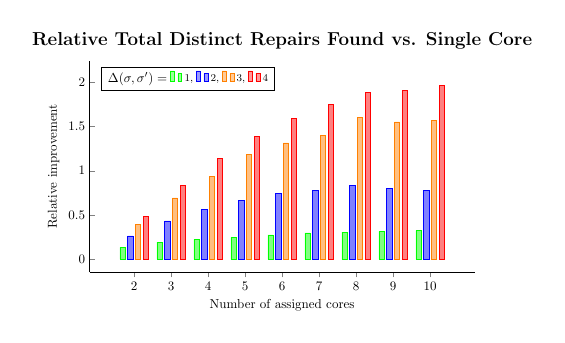
\begin{tikzpicture}[scale=0.47]
  \begin{axis}[
    legend cell align={left},
    legend style={fill opacity=0.8, draw opacity=1, text opacity=1, legend columns=-1, legend pos=north west},
    ybar,
    enlargelimits=0.15,
    legend style={at={(0.03,0.97)},anchor=north west},
    title={\Large\textbf{Relative Total Distinct Repairs Found vs. Single Core}},
    x=1cm,
    axis lines*=left,
    ylabel={Relative improvement},
    xlabel={Number of assigned cores},
    symbolic x coords={2,3,4,5,6,7,8,9,10},
    xtick=data,
    bar width=4pt,
  ]
    \addlegendimage{empty legend}
    \addlegendentry{$\Delta(\err\sigma, \sigma')=$}
    \addlegendentry{\footnotesize{$1,$}}
    \addlegendentry{\footnotesize{$2,$}}
    \addlegendentry{\footnotesize{$3,$}}
    \addlegendentry{\footnotesize{$4$}}
    \addplot[green, fill=green!50] coordinates { (2,0.1343) (3,0.1955) (4,0.2249) (5,0.2475) (6,0.2760) (7,0.2994) (8,0.3073) (9,0.3151) (10,0.3229) };
    \addplot[blue, fill=blue!50] coordinates { (2,0.2655) (3,0.4353) (4,0.5614) (5,0.6644) (6,0.7462) (7,0.7783) (8,0.8347) (9,0.8005) (10,0.7798) };
    \addplot[orange, fill=orange!50] coordinates { (2,0.3972) (3,0.6928) (4,0.9327) (5,1.1834) (6,1.3138) (7,1.3988) (8,1.6039) (9,1.5500) (10,1.5691) };
    \addplot[red, fill=red!50] coordinates { (2,0.4863) (3,0.8326) (4,1.1368) (5,1.3879) (6,1.5873) (7,1.7494) (8,1.8802) (9,1.9059) (10,1.9625) };
  \end{axis}
\end{tikzpicture}